\cleardoublepage

\chapter{Imprimerie Nationale}

%%%%%%%%%%%%%%%%%%%%%%%%%%%%%%%%%%%%%%%%%%%%%%%%%%%%%%%%%%%%%%%%%%%%%%%%%%%
%%%%%%%%%%%%%%%%%%%%%%%%%%%%%%%%%%%%%%%%%%%%%%%%%%%%%%%%%%%%%%%%%%%%%%%%%%%
%%%%%%%%%%%%%%%%%%%%%%%%%%%%%%%%%%%%%%%%%%%%%%%%%%%%%%%%%%%%%%%%%%%%%%%%%%%
%%%%%%%%%%%%%%%%%%%%%%%%%%%%%%%%%%%%%%%%%%%%%%%%%%%%%%%%%%%%%%%%%%%%%%%%%%%
%%%%%%%%%%%%%%%%%%%%%%%%%%%%%%%%%%%%%%%%%%%%%%%%%%%%%%%%%%%%%%%%%%%%%%%%%%%

\section{Le contexte}

L'objectif du projet est de concevoir une solution de gestion d'identité numérique.
Ces identités sont stockées sur des supports physiques, tels que des badges ou des cartes à puce.
Des services seront proposés à ces supports, il peut s'agir par exemple d'accès à un bâtiment, de chiffrement ou de signature de données sensibles, \ldots
\\

L'Imprimerie Nationale désire vendre cette solution à divers clients dans le but de leur produire leurs supports.
L'architecture retenue sera donc \textit{multi-tenant}, c'est-à-dire que chaque client possèdera ses propres données.
Cette solution sera hébergée à l'Imprimerie Nationale et chacun des clients pourra se connecter à l'application pour gérer ses supports et services.
\\

Ce projet est réalisé par plusieurs sociétés :
\begin{itemize}
	\item Keynectis pour l'infrastructure de gestion de clés
	\item Dictao pour l'activation des cartes à puce ;
	\item l'Imprimerie Nationale pour la personnalisation des identités ;
	\item et Sopra Group pour le développement du système de gestion d'identités.
\end{itemize}
L'équipe du projet est composé d'une quinzaine de personnes, majoritairement de l'agence de Clermont Ferrand, mais dont certains étaient rattachés à l'agence de Lyon ou Grenoble.

%%%%%%%%%%%%%%%%%%%%%%%%%%%%%%%%%%%%%%%%%%%%%%%%%%%%%%%%%%%%%%%%%%%%%%%%%%%
%%%%%%%%%%%%%%%%%%%%%%%%%%%%%%%%%%%%%%%%%%%%%%%%%%%%%%%%%%%%%%%%%%%%%%%%%%%
%%%%%%%%%%%%%%%%%%%%%%%%%%%%%%%%%%%%%%%%%%%%%%%%%%%%%%%%%%%%%%%%%%%%%%%%%%%
%%%%%%%%%%%%%%%%%%%%%%%%%%%%%%%%%%%%%%%%%%%%%%%%%%%%%%%%%%%%%%%%%%%%%%%%%%%
%%%%%%%%%%%%%%%%%%%%%%%%%%%%%%%%%%%%%%%%%%%%%%%%%%%%%%%%%%%%%%%%%%%%%%%%%%%

\section{L'administration}

L'application est divisée en divers niveaux afin de séparer les différentes fonctionnalités.
La figure \ref{niveaux_administration} représente les différents niveaux présentés dans cette section.
\begin{figure}[!h]
	\center
	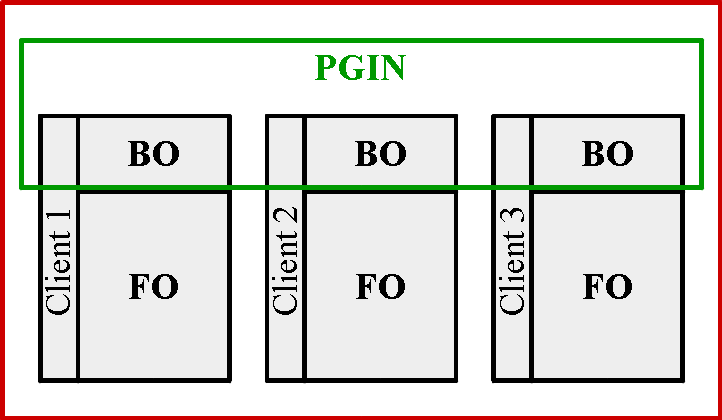
\includegraphics[width=0.8\textwidth]{img/niveaux_administration.png}
	\caption{Niveaux d'administration de l'application}
	\label{niveaux_administration}
\end{figure}

%%%%%%%%%%%%%%%%%%%%%%%%%%%%%%%%%%%%%%%%%%%%%%%%%%%%%%%%%%%%%%%%%%%%%%%%%%%
%%%%%%%%%%%%%%%%%%%%%%%%%%%%%%%%%%%%%%%%%%%%%%%%%%%%%%%%%%%%%%%%%%%%%%%%%%%
%%%%%%%%%%%%%%%%%%%%%%%%%%%%%%%%%%%%%%%%%%%%%%%%%%%%%%%%%%%%%%%%%%%%%%%%%%%

\subsection{Le Front Office}

Le \textit{Front Office} (FO) est la partie accessible par les utilisateurs finaux.
Elle propose les principales fonctionnalités principales de l'application.
Dans notre cas il s'agit des fonctions de gestion des supports : demande, validation, révocation, \ldots

% TODO détailler demande, validation, révocation

%%%%%%%%%%%%%%%%%%%%%%%%%%%%%%%%%%%%%%%%%%%%%%%%%%%%%%%%%%%%%%%%%%%%%%%%%%%
%%%%%%%%%%%%%%%%%%%%%%%%%%%%%%%%%%%%%%%%%%%%%%%%%%%%%%%%%%%%%%%%%%%%%%%%%%%
%%%%%%%%%%%%%%%%%%%%%%%%%%%%%%%%%%%%%%%%%%%%%%%%%%%%%%%%%%%%%%%%%%%%%%%%%%%

\subsection{Le Back Office}

Le \textit{Back Office} (BO) est quant à lui destinée aux administrateurs de l'application.
L'objectif de cette partie est de gérer les utilisateurs et droits, mais aussi de gérer les données "statiques" qui apparaitront dans la partie front office comme par exemple l'ensemble des supports disponibles.

Il s'agit du niveau sur lequel j'ai travaillé durant mon stage et que je vous présenterai dans ce chapitre.

%%%%%%%%%%%%%%%%%%%%%%%%%%%%%%%%%%%%%%%%%%%%%%%%%%%%%%%%%%%%%%%%%%%%%%%%%%%

\subsubsection{Administration}

Il est nécessaire que chaque client puisse administrer les proposer données qui lui sont propre, sans impacter les données des autres clients.
Pour cela un niveau "Administrateur" a été mis en place.

%%%%%%%%%%%%%%%%%%%%%%%%%%%%%%%%%%%%%%%%%%%%%%%%%%%%%%%%%%%%%%%%%%%%%%%%%%%

\subsubsection{PGIN}

L'imprimerie va produire des cartes pour l'ensemble de ses clients.
Ainsi des données seront communes à chacune des clients et il est nécessaire de pouvoir les gérer efficacement.
De plus, il est nécessaire de pouvoir administrer l'application de chacun des clients, en cas de problème ou pour effectuer des maintenances.

Dans cet objectif, un niveau "PGIN" (signifiant Plateforme de Personnalisation de l'Identité Numérique) a été mis en place afin d'administrer l'ensemble des données des clients.
Il s'agit d'un niveau "super administrateur" au niveau de l'Imprimerie Nationale.

%%%%%%%%%%%%%%%%%%%%%%%%%%%%%%%%%%%%%%%%%%%%%%%%%%%%%%%%%%%%%%%%%%%%%%%%%%%
%%%%%%%%%%%%%%%%%%%%%%%%%%%%%%%%%%%%%%%%%%%%%%%%%%%%%%%%%%%%%%%%%%%%%%%%%%%
%%%%%%%%%%%%%%%%%%%%%%%%%%%%%%%%%%%%%%%%%%%%%%%%%%%%%%%%%%%%%%%%%%%%%%%%%%%
%%%%%%%%%%%%%%%%%%%%%%%%%%%%%%%%%%%%%%%%%%%%%%%%%%%%%%%%%%%%%%%%%%%%%%%%%%%
%%%%%%%%%%%%%%%%%%%%%%%%%%%%%%%%%%%%%%%%%%%%%%%%%%%%%%%%%%%%%%%%%%%%%%%%%%%

\section{Gestion des instances}

%%%%%%%%%%%%%%%%%%%%%%%%%%%%%%%%%%%%%%%%%%%%%%%%%%%%%%%%%%%%%%%%%%%%%%%%%%%
%%%%%%%%%%%%%%%%%%%%%%%%%%%%%%%%%%%%%%%%%%%%%%%%%%%%%%%%%%%%%%%%%%%%%%%%%%%
%%%%%%%%%%%%%%%%%%%%%%%%%%%%%%%%%%%%%%%%%%%%%%%%%%%%%%%%%%%%%%%%%%%%%%%%%%%

\subsection{Présentation}

Une instance, aussi appelé niveau hiérarchique, et une entité de l'entreprise.
Les différentes instances forment une hiérarchie, représentée sous la forme d'un arbre.
L'instance racine est la compagnie et est unique pour un client donné.
Les instances sous-jacentes sont les divisions, et les feuilles sont les domaines.
La solution actuelle se limite à trois niveaux dans la hiérarchie.

À titre d'exemple, on peut représenter Sopra Group France qui est composée de divisions (Rhône-Alpes Auvergne, \ldots) qui sont elles-même composées d'agences (Clermont Ferrand, Lyon, \ldots).
La figure \ref{hierarchie_Sopra_Group} représente la hiérarchie de Sopra Group France.
\begin{figure}[!h]
	\center
	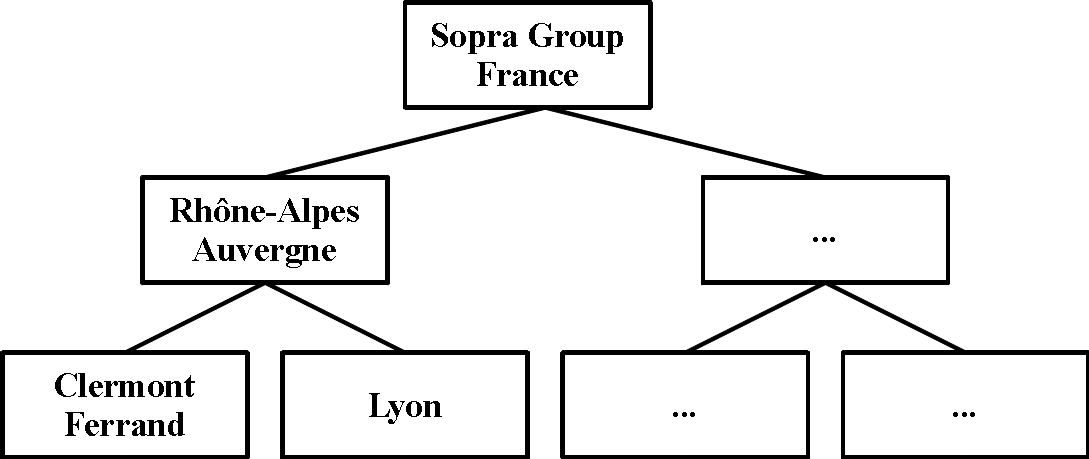
\includegraphics[width=0.8\textwidth]{img/hierarchie_Sopra_Group.png}
	\caption{Hiérarchie de Sopra Group France}
	\label{hierarchie_Sopra_Group}
\end{figure}
~~\\

%%%%%%%%%%%%%%%%%%%%%%%%%%%%%%%%%%%%%%%%%%%%%%%%%%%%%%%%%%%%%%%%%%%%%%%%%%%
%%%%%%%%%%%%%%%%%%%%%%%%%%%%%%%%%%%%%%%%%%%%%%%%%%%%%%%%%%%%%%%%%%%%%%%%%%%
%%%%%%%%%%%%%%%%%%%%%%%%%%%%%%%%%%%%%%%%%%%%%%%%%%%%%%%%%%%%%%%%%%%%%%%%%%%

\subsection{Les écrans}

J'ai tout d'abord travaillé sur la gestion des instances.
L'objectif est de pouvoir effectuer les opérations courantes (affichage, modification, création, suppression), ainsi que l'association des utilisateurs.
La figure \ref{instances_UML} est le diagramme UML des instances.
\begin{figure}[!h]
	\center
	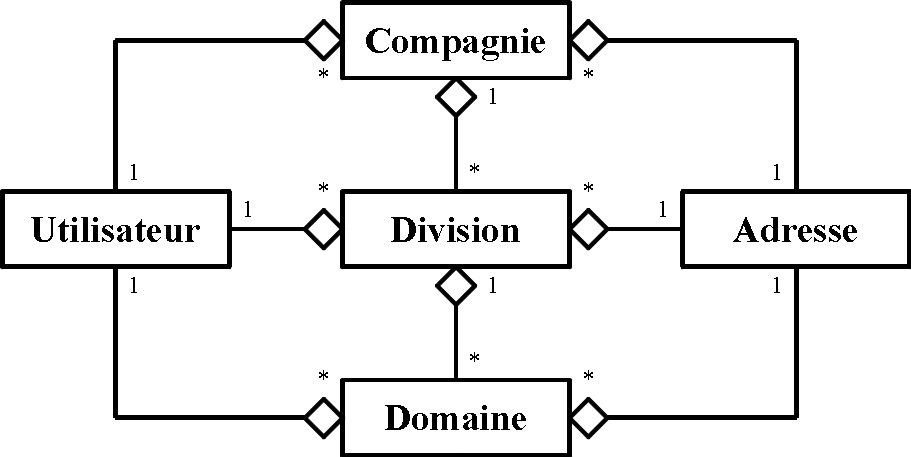
\includegraphics[width=0.8\textwidth]{img/instances_UML.png}
	\caption{Diagramme UML des instances}
	\label{instances_UML}
\end{figure}

%%%%%%%%%%%%%%%%%%%%%%%%%%%%%%%%%%%%%%%%%%%%%%%%%%%%%%%%%%%%%%%%%%%%%%%%%%%

\subsubsection{Managing}

L'écran d'accueil de la gestion affiche la hiérarchie des instances, présenté sur la figure \ref{instances_managing} qui en est une capture d'écran.
Des boutons d'action permettent d'agir sur l'instance sélectionnée.
\begin{figure}[!h]
	\center
	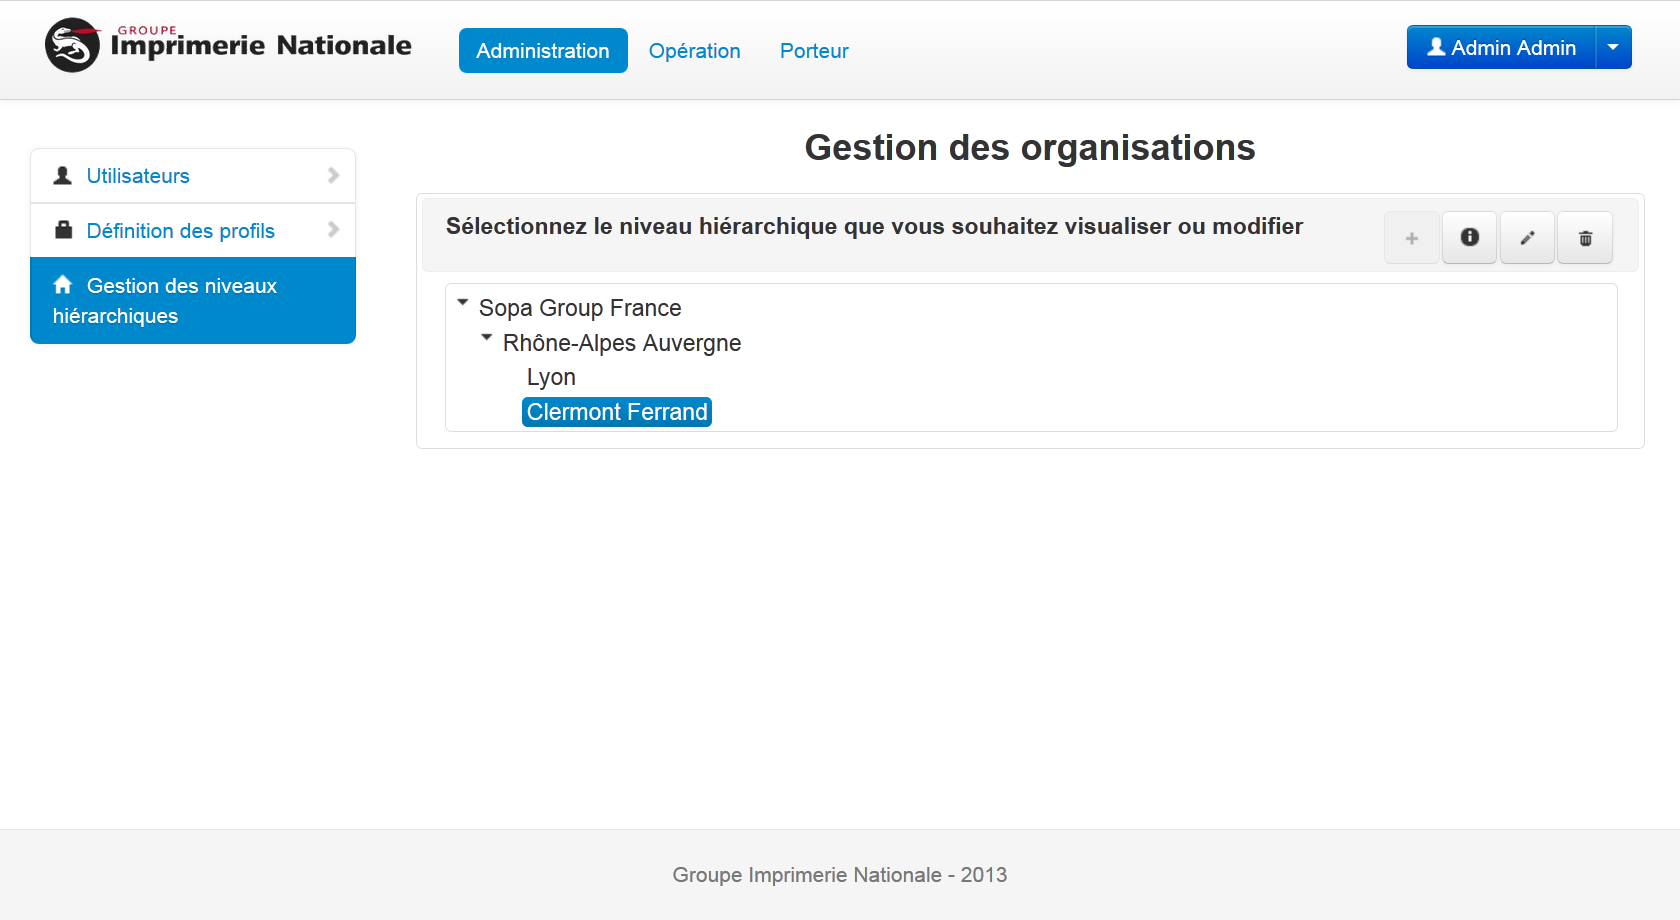
\includegraphics[width=1\textwidth]{img/instances_managing.png}
	\caption{Managing des instances}
	\label{instances_managing}
\end{figure}
~~\\

La suppression d'une instance se fait en sélectionnant une instance dans la hiérarchie de l'écran puis en cliquant sur le bouton "Supprimer".
Pour des raisons de sécurité, il est impossible de supprimer une instance si celle-ci possède des liens avec d'autres données dans la base de données.
Par exemple il est impossible de supprimer une division s'il existe des domaines sous-jacents.

%%%%%%%%%%%%%%%%%%%%%%%%%%%%%%%%%%%%%%%%%%%%%%%%%%%%%%%%%%%%%%%%%%%%%%%%%%%

\subsubsection{Affichage, modification et création}

Dans ce type d'actions, il existe deux types d'écran.
L'affichage montre simplement à l'utilisateur les valeurs des différents champs.
Les écrans de création et modification proposent quand à eux une zone de saisie, où les champs sont pré-remplies par la valeur dans le cas d'une modification.

Dans les trois cas, l'utilisateur a accès aux informations des instances parentes en cliquant sur l'onglet correspondant.
Par exemple lorsque l'on modifie une division, la division et la compagnie sont affichées (sans modification possible).
Cela permet à l'utilisateur de connaître quelle instance il manipule et où elle se situe dans la hiérarchie.
La figure \ref{instances_modification} est une capture d'écran de la fenêtre de modification d'une division.
\begin{figure}[!h]
	\center
	
\includegraphics[width=1\textwidth]{img/instances_modification.png}
	\caption{Modification d'un domaine}
	\label{instances_modification}
\end{figure}

%%%%%%%%%%%%%%%%%%%%%%%%%%%%%%%%%%%%%%%%%%%%%%%%%%%%%%%%%%%%%%%%%%%%%%%%%%%

\subsubsection{Les utilisateurs}

Chaque utilisateur de l'application est rattaché à une instance.
La modification d'une instance permet aussi d'associer de nouveaux utilisateurs ou de supprimer des nouveaux utilisateurs à l'instance.

La figure \ref{instances_utilisateurs} est l'écran d'affectation, composé de deux parties : la liste des utilisateurs disponibles avec un filtre de recherche, et la liste des utilisateurs associés.
Les deux listes sont complémentaires, c'est-à-dire que l'association d'un utilisateur à l'instance le fera passer de la liste des disponibles à la liste des associés.
L'association se fait en sélectionnant des utilisateurs dans une des liste puis en cliquant sur le bouton "flèche du haut" ou "flèche du bas" pour ajouter ou retirer des utilisateurs.
\begin{figure}[!h]
	\center
	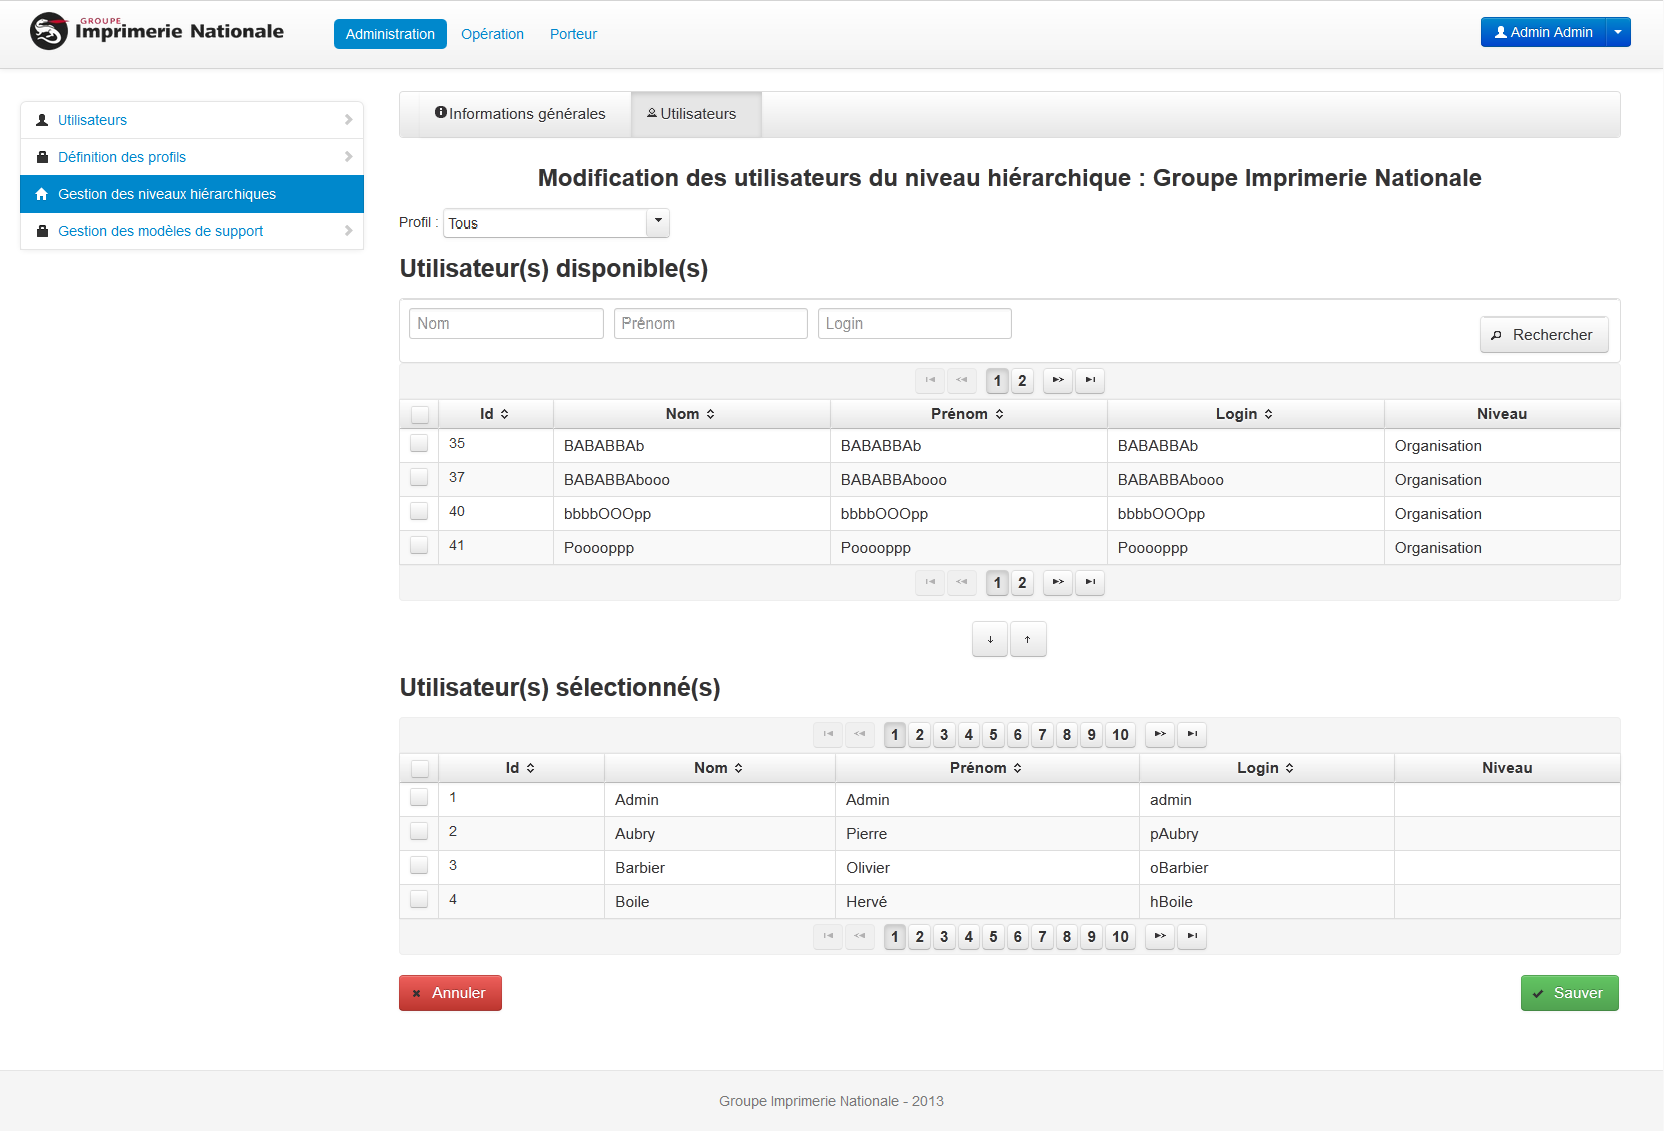
\includegraphics[width=1\textwidth]{img/instances_utilisateurs.png}
	\caption{Association d'utilisateurs à une instance}
	\label{instances_utilisateurs}
\end{figure}

%%%%%%%%%%%%%%%%%%%%%%%%%%%%%%%%%%%%%%%%%%%%%%%%%%%%%%%%%%%%%%%%%%%%%%%%%%%
%%%%%%%%%%%%%%%%%%%%%%%%%%%%%%%%%%%%%%%%%%%%%%%%%%%%%%%%%%%%%%%%%%%%%%%%%%%
%%%%%%%%%%%%%%%%%%%%%%%%%%%%%%%%%%%%%%%%%%%%%%%%%%%%%%%%%%%%%%%%%%%%%%%%%%%
%%%%%%%%%%%%%%%%%%%%%%%%%%%%%%%%%%%%%%%%%%%%%%%%%%%%%%%%%%%%%%%%%%%%%%%%%%%
%%%%%%%%%%%%%%%%%%%%%%%%%%%%%%%%%%%%%%%%%%%%%%%%%%%%%%%%%%%%%%%%%%%%%%%%%%%

\section{Gestion des profils}

%%%%%%%%%%%%%%%%%%%%%%%%%%%%%%%%%%%%%%%%%%%%%%%%%%%%%%%%%%%%%%%%%%%%%%%%%%%
%%%%%%%%%%%%%%%%%%%%%%%%%%%%%%%%%%%%%%%%%%%%%%%%%%%%%%%%%%%%%%%%%%%%%%%%%%%
%%%%%%%%%%%%%%%%%%%%%%%%%%%%%%%%%%%%%%%%%%%%%%%%%%%%%%%%%%%%%%%%%%%%%%%%%%%

\subsection{Généralités}

Les différentes restrictions dans l'application sont gérées par des droits.
En fonction des droits que possède l'utilisateur, celui-ci verra des entrées dans les menus, des boutons d'action, \ldots cachés.
Cette gestion des droits se fait finement par l'intermédiaire des profils, comme détaillé dans le chapitre précédent \ref{Gestion des droits}.
\\

L'écran d'affectation des utilisateurs est identique à celui de la figure \ref{instances_utilisateurs}.
L'écran d'affectation des droits diffère uniquement sur les données affichées car ici on y manipule des droits.

%%%%%%%%%%%%%%%%%%%%%%%%%%%%%%%%%%%%%%%%%%%%%%%%%%%%%%%%%%%%%%%%%%%%%%%%%%%
%%%%%%%%%%%%%%%%%%%%%%%%%%%%%%%%%%%%%%%%%%%%%%%%%%%%%%%%%%%%%%%%%%%%%%%%%%%
%%%%%%%%%%%%%%%%%%%%%%%%%%%%%%%%%%%%%%%%%%%%%%%%%%%%%%%%%%%%%%%%%%%%%%%%%%%

\subsection{Différents niveaux}

Il existe deux types de profils dans l'application :
\begin{itemize}
	\item les profils dits "spécifiques" qui sont propres à un client ;
	\item les profils dits "communs" qui sont présent chez l'ensemble des clients.
\end{itemize}
Leur gestion varie en fonction du niveau dans lequel il se trouve.

%%%%%%%%%%%%%%%%%%%%%%%%%%%%%%%%%%%%%%%%%%%%%%%%%%%%%%%%%%%%%%%%%%%%%%%%%%%

\subsubsection{Administration}
\label{IN_GestionDesProfils_DifférentsNiveaux_Administration}

Dans le niveau administration, propre à un client, les profils communs ont une gestion très limitée : il n'est possible de modifier que l'affectation des utilisateurs.
Ces profils sont proposés pour fournir des "profils de base" que les clients pourront affecter aux utilisateurs dans le cadre d'une utilisation simple de l'application.

Concernant les profils spécifiques, il est possible d'en créer des nouveaux, de les supprimer, et de modifier l'affectation de droits et utilisateurs.
Chaque client peut ensuite personnaliser ses accès et restrictions.

%%%%%%%%%%%%%%%%%%%%%%%%%%%%%%%%%%%%%%%%%%%%%%%%%%%%%%%%%%%%%%%%%%%%%%%%%%%

\subsubsection{PGIN}

\Jparagraph{Spécifique}
Les profils spécifiques permettent d'administrer les droits dans la partie PGIN de l'application.

\Jparagraph{Commun}
Les profils communs demandent des opérations plus complexes dans la base de données.
En effet, un profil commun est dupliqué sur l'ensemble des clients, et il est nécessaire que ces profils soient tous identiques.
Une action sur un profil commun dans le niveau PGIN devra donc être répercutée chez chacun des clients.

Une problématique importante s'est soulevée lors de l'implémentation des fonctionnalités : retrouver le profil commun.
Habituellement un profil est identifié par un identifié unique : la clé primaire.
Or lorsque l'on va créer un nouveau profil commun celui-ci n'aura pas le même identifiant dans chacune des tables, en raison du fait que les identifiants sont auto-générés.
La solution que j'ai utilisée est d'identifier le profil par une clé alternative, c'est à dire une valeur unique : le nom.
Ce nom n'est modifiable par aucun client, comme expliqué précédemment dans la partie \ref{IN_GestionDesProfils_DifférentsNiveaux_Administration}, ce qui permet d'utiliser le nom pour retrouver les différents profils communs dans les tables des clients.

%%%%%%%%%%%%%%%%%%%%%%%%%%%%%%%%%%%%%%%%%%%%%%%%%%%%%%%%%%%%%%%%%%%%%%%%%%%
%%%%%%%%%%%%%%%%%%%%%%%%%%%%%%%%%%%%%%%%%%%%%%%%%%%%%%%%%%%%%%%%%%%%%%%%%%%
%%%%%%%%%%%%%%%%%%%%%%%%%%%%%%%%%%%%%%%%%%%%%%%%%%%%%%%%%%%%%%%%%%%%%%%%%%%
%%%%%%%%%%%%%%%%%%%%%%%%%%%%%%%%%%%%%%%%%%%%%%%%%%%%%%%%%%%%%%%%%%%%%%%%%%%
%%%%%%%%%%%%%%%%%%%%%%%%%%%%%%%%%%%%%%%%%%%%%%%%%%%%%%%%%%%%%%%%%%%%%%%%%%%

\section{Résultats}

Actuellement mes différents écrans répondent aux besoins du client.
Ils proposent une partie des fonctionnalités présentes dans la partie back office de l'application permettant d'administrer les droits et les instances.

Le projet a été livré à la fin du mois d'août au client.
Actuellement en phase de qualification, l'application sera mise en production à la fin du mois de septembre pour être proposée à d'éventuelles sociétés.